\chapter{Threads and Concurrency}
Most modern applications are \textbf{multithreaded}, meaning that multiple threads run within a single application. Each thread can handle a separate task, such as \textbf{updating the display}, \textbf{fetching data}, performing \textbf{spell checking}, or \textbf{answering network requests}. Unlike \textbf{process creation}, which is heavy-weight, \textbf{thread creation} is light-weight, making it easier to simplify code and increase efficiency.

Most \textbf{kernels are also multithreaded}, which provides several benefits. \textbf{Responsiveness} is improved because a process can continue executing even if part of it is blocked, which is particularly important for user interfaces. \textbf{Resource sharing} is simpler with threads, since threads share the resources of their parent process, avoiding the complexity of shared memory or message passing. Threads are also \textbf{economical}, because creating a thread is cheaper than creating a process and thread switching has lower overhead than context switching. Finally, multithreaded processes enhance \textbf{scalability}, allowing applications to take advantage of \textbf{multicore architectures}.

\begin{figure}[H]
    \centering
    \begin{minipage}{0.5\textwidth}
        \centering
        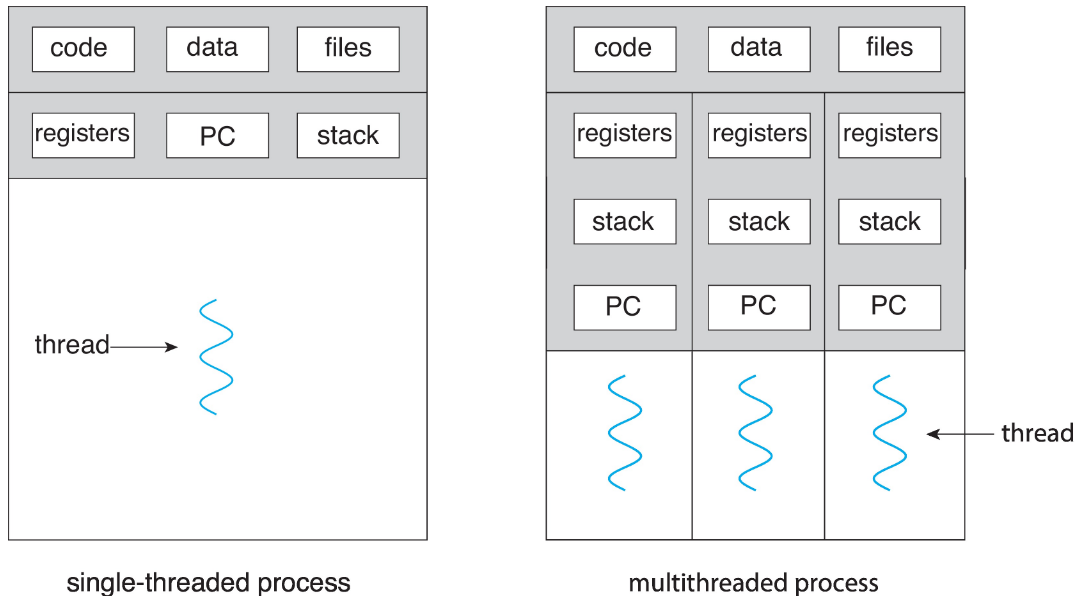
\includegraphics[width=\textwidth]{images/single_multiple_proccess.png}
        \caption{Sigle and MultiThreaded Process}
        \label{fig:Process_in_Memory}
    \end{minipage}
    \hfill
    \begin{minipage}{0.4\textwidth}
        \centering
        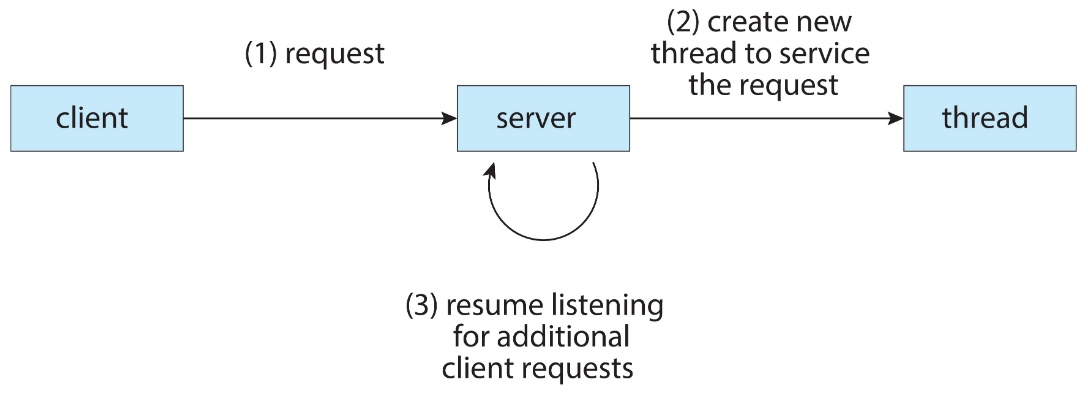
\includegraphics[width=\textwidth]{images/multiple_server.png}
        \caption{MultiThreaded Servers Architecture} 
        \label{fig:MultiThreaded_Servers_Architecture}
    \end{minipage}
    \label{fig:Threads_and_Concurrency}
\end{figure}

\section{Multicore Programming}
Multicore or multiprocessor systems put significant pressure on programmers. Key challenges include dividing activities among cores, maintaining load balance, splitting data efficiently, managing data dependencies, and performing thorough testing and debugging. In these systems, \textbf{parallelism} implies that the system can perform more than one task simultaneously, while \textbf{concurrency} refers to multiple tasks making progress over time, even on a single-core processor where the scheduler interleaves execution to provide concurrency.

There are two main types of parallelism. \textbf{Data parallelism} distributes subsets of the same data across multiple cores, performing the same operation on each subset. In contrast, \textbf{task parallelism} involves distributing threads across cores, with each thread performing a unique operation.

\begin{figure}[H]
    \centering
    \begin{minipage}{0.5\textwidth}
        \centering
        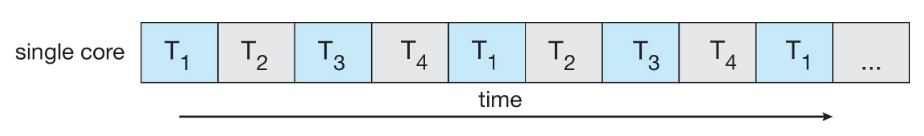
\includegraphics[width=\textwidth]{images/concurrency.png}
        \caption{Sigle and MultiThreaded Process}
        \label{fig:Concurrency_on_a_Single_Core_System}
    \end{minipage}
    \hfill
    \begin{minipage}{0.4\textwidth}
        \centering
        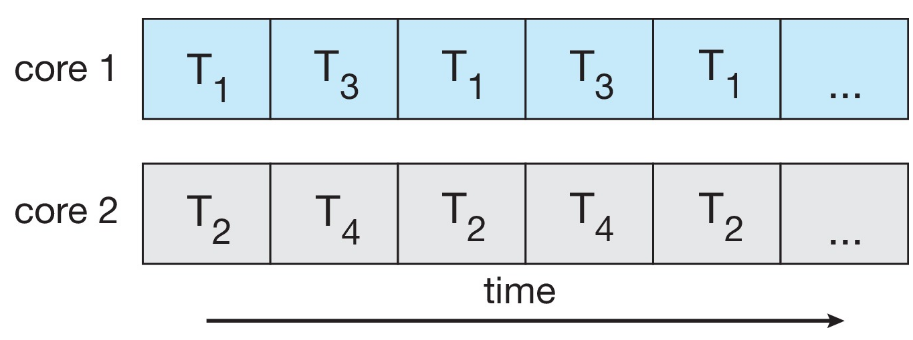
\includegraphics[width=\textwidth]{images/parallelism.png}
        \caption{Parallelism on a Multicore System} 
        \label{fig:Parallelism_on_a_Multicore_System}
    \end{minipage}
    \label{fig:Concurrency_and_Parallelism}
\end{figure}

\begin{figure}[H]
    \centering
    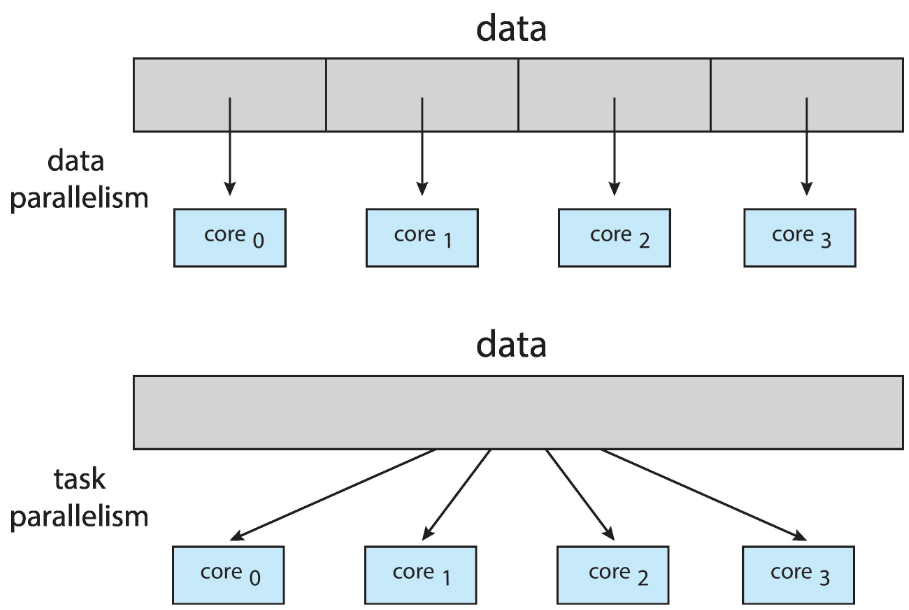
\includegraphics[width=0.5\textwidth]{images/data_task_parallelism.png}
    \caption{Data and Task Parallelism}
    \label{fig:Process States}
\end{figure}

\subsection{Amdahl's Law}

\textbf{Amdahl's Law} provides an estimate of the maximum speedup achievable when a program contains both serial and parallel components. It is given by the formula:

\begin{equation}
\text{Speedup} \leq \frac{1}{S + \frac{1-S}{N}}
\end{equation}

where $S$ is the fraction of the program that is serial and cannot be parallelized, $1-S$ is the fraction that can be parallelized, and $N$ is the number of processing cores. This law shows that the serial portion of a program limits the overall speedup. For example, if 25\% of a program is serial ($S=0.25$) and the remaining 75\% is parallel, using 2 cores results in a maximum speedup of 1.6. As $N \to \infty$, the speedup approaches $1/S$, meaning that even with infinitely many cores, the serial portion dominates the achievable performance gain. This highlights the importance of minimizing the serial fraction of a program to fully benefit from multicore architectures.

\begin{figure}[H]
    \centering
    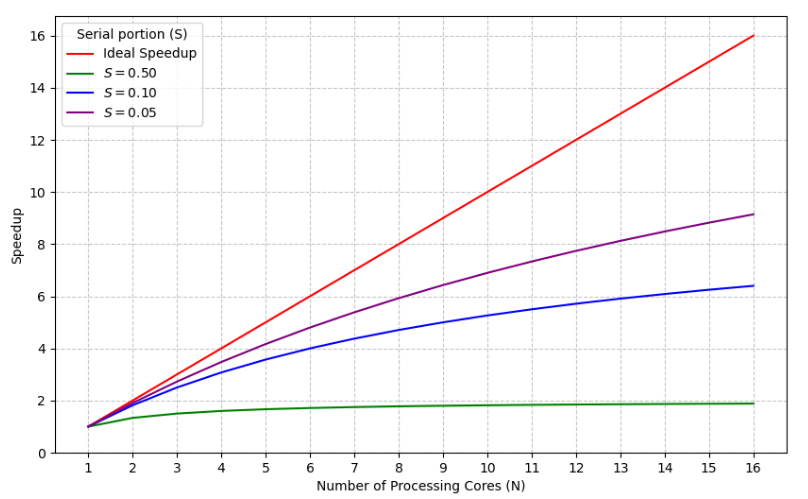
\includegraphics[width=0.5\textwidth]{images/amdahl.png}
    \caption{Amdahl's Law}
    \label{fig:Amdahls_Law}
\end{figure}

\subsection{User Threads and Kernel Threads}

\textbf{User threads} are managed entirely by a user-level threads library, such as POSIX pthreads, Windows threads, or Java threads. Management operations, scheduling, and synchronization are handled in user space, making thread creation and switching relatively lightweight. In contrast, \textbf{kernel threads} are supported directly by the operating system kernel. Almost all modern general-purpose operating systems provide kernel-level thread support, including Windows, Linux, Mac OS X, iOS, and Android. Kernel threads allow true parallel execution on multicore systems and integrate fully with the kernel's scheduling mechanisms, but they typically incur higher overhead for creation and context switching compared to user threads.

\section{Multithreading Models}
There are several approaches to mapping \textbf{user-level threads} to \textbf{kernel threads}. 

The simplest is the \textbf{Many-to-One} model, where many user-level threads are mapped onto a single kernel thread. In this model, if one thread blocks, all threads in the process are blocked because only one thread can access the kernel at a time. Consequently, multiple threads cannot run in parallel on a multicore system. This model is rarely used in modern systems, with examples including Solaris Green Threads and GNU Portable Threads.
\begin{figure}[H]
    \centering
    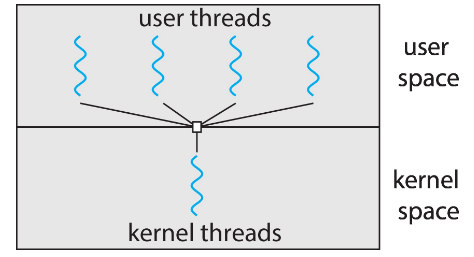
\includegraphics[width=0.3\textwidth]{images/many_to_ome.png}
    \caption{Many-to-One Model}
    \label{fig:Many_to_One_Model}
\end{figure}

The \textbf{One-to-One} model establishes a direct correspondence between each user-level thread and a kernel thread. Creating a user-level thread immediately creates a corresponding kernel thread. This model allows greater concurrency than Many-to-One because each thread can be scheduled independently by the kernel, although the number of threads per process may be restricted due to the overhead of maintaining kernel threads. Common examples of operating systems that implement this model include Windows and Linux. In this model we don't need to have a scheduler to map user threads to kernel threads, because each user thread is mapped to a kernel thread.
\begin{figure}[H]
    \centering
    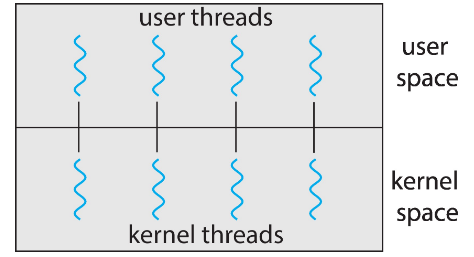
\includegraphics[width=0.3\textwidth]{images/one_to_one.png}
    \caption{One-to-One Model}
    \label{fig:One_to_One_Model}
\end{figure}

The \textbf{Many-to-Many} model allows many user-level threads to be mapped onto many kernel threads. This mapping enables the operating system to create an appropriate number of kernel threads, maximizing concurrency while controlling resource usage. An example of this model is Windows with the ThreadFiber package. While powerful, this model is not widely used. In this model we need to have a scheduler to map user threads to kernel threads, because each user thread can be mapped to any kernel thread. So this model have two scheduler, one to map user threads to kernel threads and one to map kernel threads to CPU.
\begin{figure}[H]
    \centering
    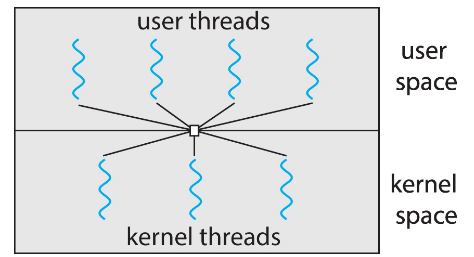
\includegraphics[width=0.3\textwidth]{images/many_to_many.png}
    \caption{Many-to-Many Model}
    \label{fig:Many_to_Many_Model}
\end{figure}

Finally, the \textbf{Two-Level} model is a variant of the Many-to-Many model. It allows user threads to be either mapped to kernel threads dynamically, as in Many-to-Many, or bound to specific kernel threads, providing additional control over scheduling and execution.
\begin{figure}[H]
    \centering
    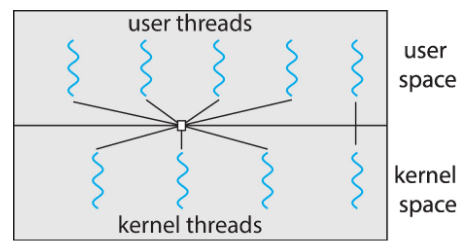
\includegraphics[width=0.3\textwidth]{images/two_level_model.png}
    \caption{Two-Level Model}
    \label{fig:Two_Level_Model}
\end{figure}

\section{Libraries and Patterns}

Thread libraries provide the programmer with an API for creating and managing threads. They can be implemented either entirely in user space or with kernel support. A widely used example is \texttt{pthreads}, which follows the POSIX standard (IEEE 1003.1c). This standard defines the expected behavior of the library, leaving the actual implementation up to the developers. \texttt{pthreads} is commonly used in UNIX-based systems such as Linux and macOS.

\subsection{POSIX Threads Example}

A simple \texttt{pthreads} program demonstrates the basic lifecycle of a thread: creation, execution, and synchronization with the main process. In the following example, a thread calculates the sum of integers from 1 up to a user-specified limit:

\begin{lstlisting}[language=C]
#include <pthread.h>
#include <stdio.h>
#include <stdlib.h>

int sum;

void *runner(void *param) {
    int upper = atoi(param);
    sum = 0;
    for (int i = 1; i <= upper; i++)
        sum += i;
    return 0;
}

int main(int argc, char *argv[]) {
    pthread_t tid;
    pthread_attr_t attr;

    pthread_attr_init(&attr);
    pthread_create(&tid, &attr, runner, argv[1]);
    pthread_join(tid, NULL);

    printf("sum = %d\n", sum);
    return 0;
}
\end{lstlisting}

\subsection{Java Threads}

Java threads are managed by the Java Virtual Machine (JVM) and typically rely on the underlying OS thread model. Threads can be created by extending the \texttt{Thread} class or by implementing the \texttt{Runnable} interface. The following example illustrates creating a simple thread using \texttt{Runnable}:

\begin{lstlisting}[language=Java]
class Task implements Runnable {
    public void run() {
        System.out.println("I am a thread.");
    }
}

Thread worker = new Thread(new Task());
worker.start();
worker.join(); // waits for the thread to complete
\end{lstlisting}

\subsection{Implicit Threading and Thread Pools}

As applications grow in complexity, explicit thread management becomes error-prone. Implicit threading, where the creation and management of threads are handled by compilers or runtime libraries, has gained popularity. Thread pools are a common pattern in implicit threading. They create a fixed number of threads that wait for tasks, improving performance by reusing existing threads rather than creating new ones for each task. In Java, the \texttt{Executors} class provides factory methods to create thread pools:

\begin{lstlisting}[language=Java]
ExecutorService pool = Executors.newCachedThreadPool();
for (int i = 0; i < numTasks; i++)
    pool.execute(new Task());
// shutdown pool after all tasks complete
pool.shutdown();
\end{lstlisting}

This approach separates the definition of tasks from the mechanics of execution, allowing better scheduling and efficient use of resources.

\subsection{Implicit Threading with OpenMP}

OpenMP is a set of compiler directives and an API for C, C++, and Fortran that simplifies parallel programming in shared-memory environments. Parallel regions can be identified using compiler pragmas, and the compiler handles the creation and management of threads. For example, a simple parallel block in C can be defined using:

\begin{lstlisting}[language=C]
#include <omp.h>
#include <stdio.h>

int main() {
    #pragma omp parallel
    {
        printf("I am a parallel region.\n");
    }
    return 0;
}
\end{lstlisting}

Similarly, loops can be executed in parallel using the \texttt{parallel for} pragma:

\begin{lstlisting}[language=C]
#pragma omp parallel for
for (int i = 0; i < N; i++) {
    c[i] = a[i] + b[i];}
\end{lstlisting}

This approach allows the programmer to express parallelism declaratively, letting the compiler and runtime handle thread management, load balancing, and scheduling, which reduces complexity and potential for errors.

\section{Issue}
When dealing with multithreaded applications, several issues arise that affect correctness and performance. One important aspect concerns the semantics of \texttt{fork()} and \texttt{exec()} system calls. The question is whether \texttt{fork()} duplicates only the calling thread or the entire set of threads within the process. Some UNIX variants actually provide two versions of \texttt{fork()}, one that duplicates all threads and one that only duplicates the calling thread. On the other hand, \texttt{exec()} behaves as usual, replacing the entire process image and therefore terminating all threads.

Signal handling is another critical issue. In UNIX systems, signals notify a process when a particular event occurs, and a signal handler is used to process it. Each signal has a default handler provided by the kernel, but the programmer can specify a user-defined handler. In single-threaded programs the signal is delivered to the process as a whole, while in multithreaded environments the delivery is less clear. A signal can be directed to the specific thread to which it applies, to all threads, to a subset of threads, or a dedicated thread can be chosen to handle all signals. The \texttt{pthreads} library provides a per-thread signaling function:

\begin{lstlisting}[language=C]
int pthread_kill(pthread_t thread, int sig);
\end{lstlisting}

Thread cancellation is another delicate aspect, as it concerns the termination of a thread before it finishes execution. The thread targeted for termination is called the target thread. Two main approaches exist: asynchronous cancellation, which forces immediate termination, and deferred cancellation, which allows the target thread to check periodically if it should be cancelled. In \texttt{pthreads}, thread cancellation can be implemented as follows:

\begin{lstlisting}[language=C]
pthread_t tid;
/* create the thread */
pthread_create(&tid, 0, worker, NULL);
/* do some work */
/* cancel the thread */
pthread_cancel(tid);
/* wait for the thread to terminate */
pthread_join(tid, NULL);
\end{lstlisting}

The actual cancellation depends on the thread’s state and configuration. If cancellation is disabled, the request remains pending until it is re-enabled. The default mode is deferred, which requires the thread to reach a cancellation point such as \texttt{pthread\_testcancel()}. Once cancellation occurs, a cleanup handler is invoked. On Linux systems, thread cancellation is managed internally through signals.

Thread-local storage (TLS) provides each thread with its own copy of a variable, which is useful in scenarios where thread creation is not directly controlled, such as when using thread pools. Unlike local variables, which exist only within a single function invocation, TLS persists across calls but remains unique to each thread. In Java this mechanism is provided by the \texttt{ThreadLocal<T>} class, while in \texttt{pthreads} it is implemented with the type \texttt{pthread\_key\_t}. Additionally, the GCC compiler offers the keyword \texttt{\_\_thread} for declaring thread-local data.

Finally, scheduler activations address the need for communication between user-level thread libraries and the kernel in models such as many-to-many or two-level threading. The idea is to use lightweight processes (LWPs), which act as virtual processors that user threads can be scheduled onto. Each LWP is attached to a kernel thread, and scheduler activations provide \emph{upcalls}, which are communication mechanisms from the kernel to the thread library. This allows the application to maintain the correct number of kernel threads dynamically, improving flexibility and performance in managing parallelism.
